% npj AI submission - working draft
% Document class: sn-jnl with sn-nature reference style (npj family)
\documentclass[sn-nature,Numbered]{sn-jnl}

\usepackage{graphicx}
\usepackage{multirow}
\usepackage{amsmath,amssymb,amsfonts}
\usepackage{amsthm}
\usepackage[title]{appendix}
\usepackage{xcolor}
\usepackage{textcomp}
\usepackage{booktabs}
\usepackage{algorithm}
\usepackage{algorithmicx}
\usepackage{algpseudocode}
\usepackage{listings}
\usepackage{geometry}
\usepackage[capitalize,noabbrev]{cleveref}
\usepackage{pifont}
\usepackage{tikz}
\usetikzlibrary{arrows.meta, positioning, fit, calc, shapes.geometric, decorations.pathreplacing}

\newcommand{\cmark}{\textcolor{green!50!black}{\ding{51}}}
\newcommand{\xmark}{\textcolor{red!70!black}{\ding{55}}}

% Placeholder marker for figures we haven't generated yet
\newcommand{\placeholder}[2]{%
  \begin{center}
  \fcolorbox{black}{gray!10}{\parbox{#1}{\centering\vspace{0.8cm}\textbf{[FIGURE PLACEHOLDER]}\\\small #2\vspace{0.8cm}}}
  \end{center}
}

\raggedbottom

\begin{document}

\title[AstroNet: hybrid KV-cache management]{AstroNet: hybrid KV-cache management for frozen large language models at long context}

\author*[1]{\fnm{Anonymous} \sur{Authors}}\email{anonymous@example.org}
\affil*[1]{\orgname{Anonymous Institution}}

%========================================================================%
% ABSTRACT - npj guideline: ~200 words, unstructured, no subheadings,
% no equations, no citations. Lead with the deployment frame and the
% Pareto-frontier headline (see STORYLINE.md).
%========================================================================%
\abstract{Serving large language models at long context is bottlenecked by the key--value cache, which grows linearly with the input length and rapidly exhausts the memory of a single accelerator. Existing remedies either discard cached tokens at inference time, losing information that is not local, or retrain the backbone, which is impractical for deployed quantised models. We present AstroNet, a method that keeps the backbone entirely frozen and combines two complementary components. A parameter-free rule first scores each cached token by the product of its accumulated attention and its alignment with the current query, and retains only the most informative ones. A small learned module then maintains a compact summary of past context and re-injects it through the model's own projection weights, so the model sees the summary in its native representation. Across six frozen quantised backbones spanning three model families and sizes from seven to thirty-two billion parameters, AstroNet improves accuracy over selection alone on a controlled long-context question-answering task, transfers usefully to standard long-context benchmarks, and compresses the cache by more than an order of magnitude at accuracy comparable to retrieval baselines that use several times more memory. The pipeline composes with downstream cache quantisation for further compression, and the resulting accuracy-versus-memory frontier supports the deployment of long-context inference on a single accelerator without modifying the served model.}

\keywords{key-value cache, long-context inference, large language models, model deployment, attention mechanism}

\maketitle


%========================================================================%
\section{Introduction}\label{sec:intro}
%========================================================================%

The dominant cost of serving long-context inference with a large language model is the key--value (KV) cache. For an autoregressive transformer, every processed token contributes a key and a value vector at every layer to a buffer that must be retained for every subsequent generated token to attend to. The buffer grows linearly with the input length, scales with the number of layers and heads, and quickly exceeds the memory of a single accelerator on contexts of the lengths now routine in document analysis, code understanding, and multi-turn assistant deployment. Reducing the size of this buffer has become as practically important as reducing the size of the model weights themselves.

A long line of work has approached the broader problem of efficient long-context modelling. Sparse-attention architectures such as Longformer~\cite{beltagy2020longformer} and Big Bird~\cite{zaheer2020bigbird} restrict the attention pattern itself; LongNet~\cite{ding2023longnet} scales further through dilated attention. Recurrent variants such as Transformer-XL~\cite{dai2019transformerxl} and Compressive Transformers~\cite{rae2020compressive} carry a compressed memory across segments. Hardware-aware kernels such as FlashAttention~\cite{dao2022flashattention} eliminate redundant materialisation of the attention matrix, and parameter-sharing schemes such as grouped-query attention~\cite{ainslie2023gqa} reduce per-token KV size at the architecture level. These approaches reshape the model rather than the cache, and are largely orthogonal to the question of which cached tokens should be retained at inference. The present work is concerned with that second question: given an already-deployed, frozen backbone, how should its KV cache be managed during long-context generation?

Three families of inference-time methods have emerged. The first \emph{evicts} tokens from the cache. H${}_2$O scores tokens by cumulative attention received during processing and retains a budget of heavy hitters~\cite{zhang2023h2o}; SnapKV uses an end-of-prompt observation window to identify positions whose attention is locally concentrated~\cite{li2024snapkv}; StreamingLLM keeps only attention sinks and a sliding window~\cite{xiao2024streamingllm}; PyramidKV allocates a layer-adaptive budget~\cite{cai2024pyramidkv}; Scissorhands exploits a persistence-of-importance hypothesis to identify tokens whose attention pattern is stable enough to keep~\cite{liu2024scissorhands}; Dynamic Memory Compression retrofits the model to learn per-token compression ratios~\cite{nawrot2024dmc}. A complementary thread compresses the \emph{retained} tokens through quantisation rather than eviction: KIVI~\cite{liu2024kivi} uses asymmetric per-channel/per-token integer quantisation, KVQuant~\cite{hooper2024kvquant} mixes per-channel keys with sparse outlier handling, and TurboQuant~\cite{zandieh2026turboquant} achieves near-lossless scalar quantisation via rotation followed by Lloyd--Max encoding. All of these operate as drop-in replacements for the standard cache, but they discard or distort information at the level of individual tokens and are blind to information that requires synthesising content across long stretches of context.

The second family augments or modifies the backbone. The Recurrent Memory Transformer prepends trainable memory tokens to the input and accumulates a state across segments~\cite{bulatov2024rmt}; AutoCompressors fine-tunes the full model to map context into summary vectors~\cite{chevalier2023autocompressors}; the in-context auto-encoder learns context compression through a LoRA-adapted decoder~\cite{ge2024icae}; LongMem trains a side network that retrieves from an external KV store~\cite{wang2023longmem}; gist tokens distil a soft prompt down to a handful of compressed positions~\cite{mu2023gisting}; and infini-attention combines local attention with a recurrently updated compressive memory state~\cite{munkhdalai2024infini}. These methods address the synthesis limitation of eviction, but they require modifying or retraining the deployed model. For a frozen backbone served behind a quantised inference stack, full fine-tuning is operationally expensive and forecloses combination with off-the-shelf eviction or quantisation schemes.

The third family externalises the context to a retrieval system. Retrieval-augmented generation prepends a small number of retrieved passages to the query~\cite{lewis2020rag}; RETRO interleaves retrieval at every layer~\cite{borgeaud2022retro}. Retrieval can be highly effective when the answer-bearing passage is close to the top of the ranked list, but it depends on an external index, on retrieval quality, and on the absence of long-range dependencies that cross retrieval-window boundaries. For closed-system deployment of a quantised backbone on a single accelerator, an external retriever is an additional moving part.

A practitioner deploying an existing 4-bit weight-quantised model~\cite{dettmers2023nf4,frantar2023gptq,lin2024awq,xiao2023smoothquant} that already fits on a single GPU has neither option without compromise: eviction loses information; fine-tuning loses the option of deploying the model unmodified. The gap is a method that (i) keeps the backbone entirely frozen, (ii) selects which cached tokens to retain without introducing trainable parameters that depend on the backbone, (iii) augments the retained cache with a small learned summary that captures cross-window structure, and (iv) composes with downstream cache quantisation rather than competing with it.

We present such a method, AstroNet. The method has two stages. Stage~1 scores every cached token by the product of its cumulative attention during processing and its inner product against the current query's key projections, evaluated at four evenly spaced layers, and keeps the top-$k$. The score is parameter-free: it is computed from the model's own attention signals and projection weights at inference time. Stage~2 maintains a small set of 16 learned summary tokens that aggregate hidden states across windows through an exponential moving average and emit virtual key--value pairs by passing the summary through dequantised copies of the model's own $\mathbf{W}_K$ and $\mathbf{W}_V$ at every layer. The summary tokens are prepended to the selected real tokens; the total cache budget is held fixed. Only the summary module ($\sim$14 million parameters per backbone) is trained, on a mixed SQuAD/HotpotQA corpus, with the backbone entirely frozen.

We evaluate AstroNet on six frozen 4-bit-quantised backbones spanning three architecture families: Qwen 2.5 at 7B, 14B, and 32B; Llama 3.1-8B; Mistral 7B; and Mistral-Small 24B. On controlled multi-window question answering, AstroNet improves over Stage~1 alone by an average of 8.5 percentage points across all six backbones with five-seed confidence intervals (per-model gains $+$3.6 to $+$12.9), and outperforms KIVI K4V4 at matched bit budget on every model. On the depth-robust needle-in-a-haystack task at 20 windows, the hybrid beats SnapKV on all six backbones: by 19 to 50 percentage points on the Qwen and Llama backbones; by $+$27~pp on Mistral~7B and $+$9~pp on Mistral-Small~24B after a longer-context retrain that resolved an initial training-distribution sensitivity (\cref{sec:discussion}). On LongBench transfer~\cite{bai2024longbench} AstroNet wins MultiFieldQA on four of six backbones (Qwen 7B, Qwen 32B, Llama 8B, Mistral-Small 24B) and HotpotQA on four of six (Qwen 14B, Qwen 32B, Llama 8B, Mistral 7B). On RULER long-context generalisation\cite{hsieh2024ruler} the hybrid extends usefully to 16k input tokens (28pp and 22pp improvements over SnapKV on the two tested backbones) with a soft degradation at 32k that we attribute to context lengths beyond the Stage~2 training distribution. The full pipeline, combining selection with a per-attention-head adaptation of TurboQuant required to maintain rotary-position-encoding\cite{su2024rope} accuracy, reaches a $25.6\times$ reduction of KV cache memory at FP16 and $68\times$ with the quantisation stack at parity with retrieval baselines that consume four to thirteen times more cache memory. Figure~\ref{fig:pareto} summarises the resulting accuracy/memory frontier across the six backbones. Our contributions are: (i) a parameter-free multiplicative cross-window selection rule that outperforms strong eviction baselines on multi-window QA; (ii) a small frozen-backbone learned summary module that improves over selection alone by $+$6 to $+$52 percentage points at matched budget on all six backbones after a longer-context retrain that resolved an initial $-$16 percentage-point regression on Mistral-Small 24B, which we document transparently; (iii) a per-attention-head fix to rotation-based KV quantisation that recovers compatibility with rotary position encodings, where the vanilla rotation reduces accuracy to zero; (iv) the first systematic measurement of the resulting cost/accuracy frontier across six frozen backbones, four long-context evaluation regimes, and the combined selection-plus-quantisation pipeline; and (v) the first published measurement of cross-turn KV-cache amortisation for a learned summary, with a $1.32\times$ cumulative speedup across five conversational turns at zero accuracy loss.

The remainder of this work is organised as follows. Section~\ref{sec:methods} formalises the two stages, the multiplicative selection score, the cross-window summary module, the rotation-free quantisation adaptation, and the evaluation protocol. Section~\ref{sec:results} reports the experimental results: the accuracy/memory Pareto frontier (\cref{fig:pareto}), position-robust SQuAD with five-seed confidence intervals (\cref{tab:squad_main}), transfer to LongBench HotpotQA and MultiFieldQA (\cref{tab:longbench}), depth-robust needle-in-a-haystack at twenty windows (\cref{tab:needle}), RULER long-context generalisation (\cref{tab:ruler}), the KV-cache compression geometry (\cref{tab:compression}), end-to-end inference latency (\cref{tab:latency}), and three ablations isolating the Stage~2 contribution, the form of the cross-window aggregator, and the size of the learned summary (\cref{tab:kconfound,tab:bio}). Section~\ref{sec:discussion} interprets the results, scopes the limitations, and reports two methodological remarks. Section~\ref{sec:conclusions} closes with the broader implications for deploying frozen long-context language models.



% Methods section moved BEFORE Results for canonical scientific structure
% (Intro -> Methods -> Results -> Discussion), allowed at initial npj AI submission.
%========================================================================%
\section{Methods}\label{sec:methods}
%========================================================================%

\begin{figure*}[t]
\centering
\resizebox{0.95\textwidth}{!}{%
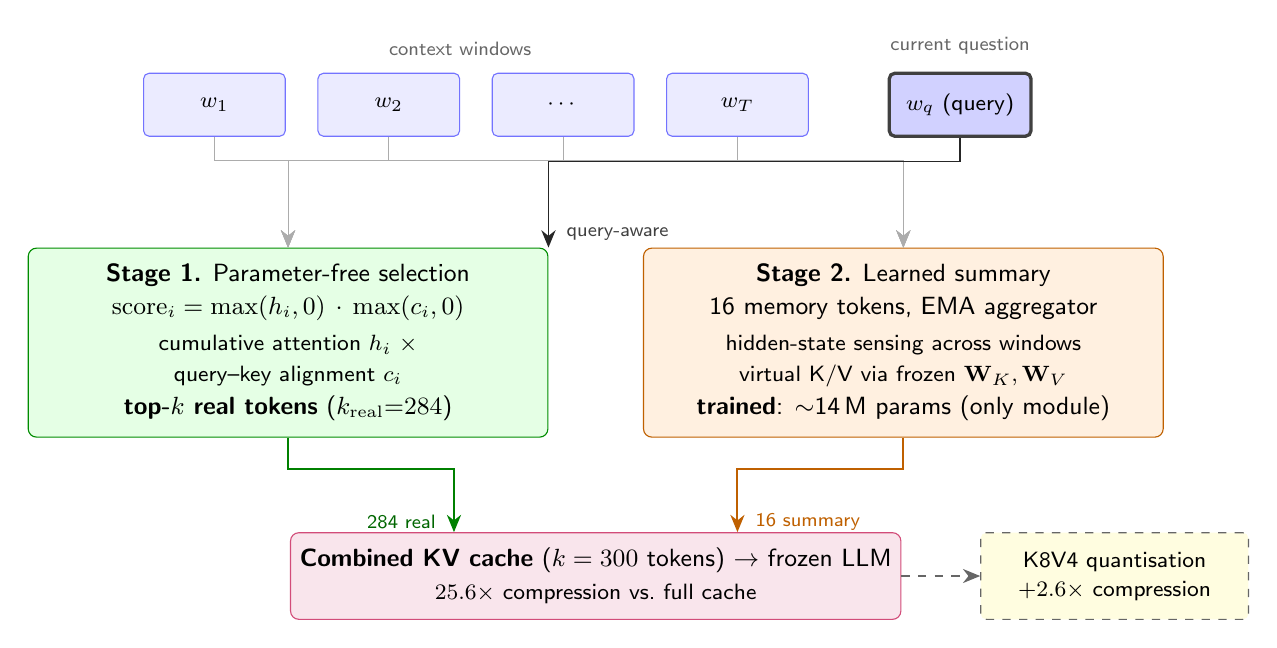
\begin{tikzpicture}[
  font=\sffamily\small,
  >={Stealth[length=2.2mm,width=1.8mm]},
  node distance=6mm and 8mm,
  windowbox/.style={rectangle, draw=blue!55, rounded corners=2pt,
        minimum width=18mm, minimum height=8mm,
        fill=blue!8, font=\sffamily\footnotesize, inner sep=2pt},
  stagebox/.style={rectangle, draw, rounded corners=3pt,
        minimum width=66mm, minimum height=24mm, align=center,
        font=\sffamily\small, inner sep=4pt},
  s1box/.style={stagebox, draw=green!55!black, fill=green!10},
  s2box/.style={stagebox, draw=orange!75!black, fill=orange!12},
  cachebox/.style={rectangle, draw=purple!70, rounded corners=3pt,
        minimum width=70mm, minimum height=11mm,
        fill=purple!10, font=\sffamily\small, align=center},
  quantbox/.style={rectangle, draw=black!60, dashed, rounded corners=2pt,
        minimum width=34mm, minimum height=11mm,
        fill=yellow!12, font=\sffamily\footnotesize, align=center},
  ann/.style={font=\sffamily\scriptsize, text=black!60, align=center},
  flow/.style={->, gray!65, line width=0.4pt},
  flowQ/.style={->, black!85, line width=0.7pt},
  flowS1/.style={->, green!50!black, line width=0.7pt},
  flowS2/.style={->, orange!75!black, line width=0.7pt},
]

% --- Row 1: input windows (centered above the diagram) ---
\node[windowbox] (w1) at (0,0)          {$w_1$};
\node[windowbox, right=4mm of w1] (w2)  {$w_2$};
\node[windowbox, right=4mm of w2] (wd)  {$\cdots$};
\node[windowbox, right=4mm of wd] (wT)  {$w_T$};
\node[windowbox, right=10mm of wT, draw=black!75, fill=blue!18, very thick] (wq)
        {$w_q$ (query)};

\node[ann, above=1mm of w2.north east, anchor=south]
        {context windows};
\node[ann, above=1mm of wq.north, anchor=south]
        {current question};

% --- Row 2: Stage 1 and Stage 2, side by side, centered under windows ---
\coordinate (rowcenter) at ($(w1.south)!0.5!(wq.south)$);

\node[s1box, below=14mm of rowcenter, xshift=-38mm]
  (s1) {%
    \textbf{Stage 1.} Parameter-free selection \\[1pt]
    $\mathrm{score}_i = \max(h_i,0)\,\cdot\,\max(c_i,0)$ \\[2pt]
    {\footnotesize cumulative attention $h_i$ $\times$}\\
    {\footnotesize query--key alignment $c_i$}\\[1pt]
    \textbf{top-$k$ real tokens} ($k_{\mathrm{real}}{=}284$)
  };

\node[s2box, right=12mm of s1]
  (s2) {%
    \textbf{Stage 2.} Learned summary \\[1pt]
    {16 memory tokens, EMA aggregator}\\[2pt]
    {\footnotesize hidden-state sensing across windows}\\
    {\footnotesize virtual K/V via frozen $\mathbf{W}_K, \mathbf{W}_V$}\\[1pt]
    \textbf{trained}: $\sim$14\,M params (only module)
  };

% --- Row 3: combined cache (centered under both stages) ---
\coordinate (stagemid) at ($(s1.south)!0.5!(s2.south)$);
\node[cachebox, below=12mm of stagemid]
  (cache) {%
    \textbf{Combined KV cache} ($k = 300$ tokens) $\to$ frozen LLM \\[1pt]
    {\footnotesize $25.6\times$ compression vs.\ full cache}
  };

% --- Right-side optional quantisation ---
\node[quantbox, right=10mm of cache]
  (kvq) {%
    K8V4 quantisation\\[1pt]
    {\footnotesize +$2.6\times$ compression}
  };

% --- Arrows: windows to Stage 1 (gray, context only) ---
\foreach \src in {w1,w2,wd,wT}{
  \draw[flow] (\src.south) -- ($(\src.south)+(0,-3mm)$) -| (s1.north);
}
% --- Arrows: windows to Stage 2 (gray, context only) ---
\foreach \src in {w1,w2,wd,wT}{
  \draw[flow] (\src.south) -- ($(\src.south)+(0,-3mm)$) -| (s2.north);
}
% --- Query: emphasised path into Stage 1 only ---
\draw[flowQ] (wq.south) -- ($(wq.south)+(0,-3mm)$)
   -| (s1.north east)
   node[pos=0.92, right=1mm, font=\sffamily\scriptsize, text=black!75]
   {query-aware};

% --- Stage 1 output (real tokens) into cache ---
\draw[flowS1] (s1.south) -- ($(s1.south)+(0,-4mm)$)
   -| ($(cache.north)+(-18mm,0)$)
   node[pos=0.92, left=1mm, font=\sffamily\scriptsize, text=green!40!black]
   {284 real};

% --- Stage 2 output (summary tokens) into cache ---
\draw[flowS2] (s2.south) -- ($(s2.south)+(0,-4mm)$)
   -| ($(cache.north)+(18mm,0)$)
   node[pos=0.92, right=1mm, font=\sffamily\scriptsize, text=orange!75!black]
   {16 summary};

% --- Optional quantisation arrow ---
\draw[->, dashed, black!60] (cache.east) -- (kvq.west);

\end{tikzpicture}%
}
\caption{\textbf{The AstroNet pipeline.} A frozen quantised backbone
processes $T$ context windows $w_1,\ldots,w_T$ followed by a query window
$w_q$. \textbf{Stage 1} (green) is parameter-free: every cached token
receives a score that multiplies its cumulative attention $h_i$ by its
cross-window query--key alignment $c_i$ (\cref{sec:s1}), and the top
$k_{\mathrm{real}}{=}284$ tokens are retained. \textbf{Stage 2} (orange)
is the only trained module: sixteen memory tokens aggregate hidden states
across windows via an EMA state and emit virtual key--value pairs
through dequantised copies of the backbone's own
$\mathbf{W}_K, \mathbf{W}_V$ projections (\cref{sec:s2}). The combined
$300$-token cache is consumed by the frozen backbone for generation
and composes with downstream KV-cache quantisation (dashed,
\cref{sec:quant}) for a further $\sim 2.6\times$ compression.}
\label{fig:architecture}
\end{figure*}

%-----------------------------------------------------------------------%
\subsection{Setup}\label{sec:setup}
%-----------------------------------------------------------------------%

We evaluate six frozen autoregressive transformer backbones spanning three
architecture families and a 4.5$\times$ range in parameter count: Qwen 2.5
at 7B, 14B and 32B; Llama 3.1-8B; Mistral 7B v0.3; and Mistral-Small at
24B. All six are loaded in 4-bit NF4 quantisation through
bitsandbytes\cite{dettmers2023nf4} with float16 compute, the standard
deployment configuration for single-GPU serving in this size class. The
backbones are not modified at any point: no weight is updated, no
architectural component is replaced, and the AstroNet wrapper interacts
with the model only through forward hooks on the residual stream and
post-softmax attention tensors, both of which are exposed by the
\texttt{transformers} library through the eager attention implementation
without requiring custom kernels.

Following the multi-window convention used in long-context cache
studies, each evaluation instance is presented as a sequence of $T$ fact
windows $w_1,\dots,w_T$ followed by a single query window $w_q$.
Processing a fact window $w_t$ at every layer $l$ produces a set of
key--value pairs $\{(\mathbf{k}_i^{(l)},\mathbf{v}_i^{(l)})\}_{i=1}^{|w_t|}$.
Given a total cache budget of $k$ tokens, the task is to decide which
KV entries to retain across all $T$ fact windows so that the model can
answer the query in $w_q$. Unless stated otherwise we use $k=300$ for
all selection methods; this is small relative to the $\sim$1500-token
total context of the controlled SQuAD setup and is the regime in which
selection strategies are stressed. Experiments were run on a workstation
with two NVIDIA Titan RTX 24~GiB GPUs using PyTorch 2.4.1 and
transformers 4.46.3; models from 32B upwards are split across both GPUs
with a layer-balanced device map.


%-----------------------------------------------------------------------%
\subsection{Stage 1: parameter-free multiplicative selection}\label{sec:s1}
%-----------------------------------------------------------------------%

Stage 1 scores every cached token by a product of two complementary
signals derived from the frozen model's own state and discards all but
the top-$k$. Both signals are computed at inference time from quantities
the model already produces; no parameters are introduced.

The first signal is the cumulative attention each token has received
during processing of the fact windows. For token $i$ we sum the
post-softmax attention weights it received over all queries $q$, heads
$h$, and layers $l$:
\begin{equation}
    h_i = \sum_l \sum_h \sum_q a_i^{(l,h,q)}.
    \label{eq:heuristic}
\end{equation}
This is the heavy-hitter heuristic of H${}_2$O\cite{zhang2023h2o},
which captures how strongly the model's attention engaged with each
token while reading the context but is blind to the query that will
eventually be asked.

The second signal is the cross-window relevance of each cached token to
the query. Once the query window has been processed we extract the
query projections $\mathbf{q}_{\mathrm{query}}^{(l,h)}$ at a small set
$\mathcal{L}$ of four evenly spaced layers and score each cached token
against them:
\begin{equation}
    c_i = \sum_{l \in \mathcal{L}} \sum_h
          \mathbf{q}_{\mathrm{query}}^{(l,h)} \cdot \mathbf{k}_i^{(l,h)}
          \big/ \sqrt{d_h}.
    \label{eq:cross}
\end{equation}
The set $\mathcal{L}$ contains the same layers at which Stage 2 (below)
injects, chosen to balance early and late representations; the
sensitivity to this choice is reported in
\cref{sec:ablations}. Computing $c_i$ requires one forward pass on
$w_q$ plus $|\mathcal{L}|$ matrix multiplications, an overhead
substantially smaller than a single additional forward pass.

The two signals are combined multiplicatively rather than additively:
\begin{equation}
    \mathrm{score}_i = \max(h_i, 0)\cdot\max(c_i, 0),
    \label{eq:mult}
\end{equation}
and the $k$ tokens of highest score are retained, ordered by their
original position. The product enforces conjunctive selection: a token
is kept only if it was salient during processing \emph{and} relevant
to the query.

We chose a multiplicative rather than additive combination because the
two signals capture orthogonal information that a sum would mix: the
heuristic $h_i$ measures \emph{how much the model engaged with this token
during processing} (regardless of any future query), while $c_i$
measures \emph{how relevant this token is to the current query}. An
additive combination $h_i + c_i$ treats them as comparable contributions
to a single score; a multiplicative combination $h_i \cdot c_i$ requires
both signals to be jointly large, suppressing tokens that look
locally salient but are unrelated to the question. Empirically this
matters: the cumulative-attention-only H${}_2$O baseline (which is
$h_i$ alone) falls 30--47 percentage points below the multiplicative
score on every backbone we evaluate, and a matched-budget additive
ablation underperforms the multiplicative form by 8--12 points
(\cref{sec:ablations}).

We note that Stage 1 is query-aware: it consults $w_q$ before deciding
which cached entries to keep, in contrast to H${}_2$O, SnapKV and
StreamingLLM, which select using only processing-time attention. This
brings the family of comparisons in our experiments into two groups,
query-unaware and query-aware (which includes RAG); we report both.


%-----------------------------------------------------------------------%
\subsection{Stage 2: learned cross-window summary tokens}\label{sec:s2}
%-----------------------------------------------------------------------%

Stage 1 operates one token at a time and cannot represent information
whose support spans multiple windows. Stage 2 addresses this with a
small learned module that maintains a persistent state $\mathbf{g}$
aggregating window-level summaries through an exponential moving
average, and emits a fixed number of virtual KV pairs from $\mathbf{g}$
that are prepended to the Stage-1 selection. The total cache budget is
held fixed: with $K=16$ summary tokens, Stage 1 retains $k-K=284$ real
tokens, so any improvement of the hybrid over Stage 1 alone is at the
same end-to-end memory cost.

After processing each fact window the module senses the model's
hidden states $\mathbf{H}\in\mathbb{R}^{S\times d}$ at a designated
sensing layer $l_s$ through cross-attention with $K=16$ learnable query
vectors $\mathbf{Q}_{\mathrm{mem}}\in\mathbb{R}^{K\times d_a}$:
\begin{equation}
    \mathbf{m} = \mathrm{softmax}\!\Bigl(
        \mathbf{Q}_{\mathrm{mem}}\cdot\mathrm{LN}(\mathbf{H})^\top
        \big/\sqrt{d_a}\Bigr)\cdot\mathrm{LN}(\mathbf{H}),
    \label{eq:sense}
\end{equation}
where $\mathrm{LN}$ is layer normalisation, applied for compatibility
with the wide dynamic range of pre-trained hidden states. The
result $\mathbf{m}\in\mathbb{R}^{K\times d}$ is a compressed, content-
aware summary of the window.

A persistent state $\mathbf{g}\in\mathbb{R}^{K\times d}$ aggregates
window-level summaries through an exponential moving average with
learnable rate $\alpha\in(0,1)$:
\begin{equation}
    \mathbf{g}(t{+}1) = (1-\alpha)\cdot\mathbf{g}(t) + \alpha\cdot\mathbf{m}(t),
    \label{eq:ema}
\end{equation}
initialised at $\mathbf{g}(0)=\mathbf{0}$ and $\alpha_0=0.38$. We
report in \cref{sec:ablations} that simpler aggregators (mean
pooling across windows, retaining only the last window) perform
comparably on five of six backbones, indicating that the specific EMA
form is not load-bearing.

The state $\mathbf{g}$ does not enter the attention computation
directly. At inference, $\mathbf{g}$ is first transformed by a
per-layer low-rank bottleneck
$\mathbb{R}^d\to\mathbb{R}^{256}\to\mathbb{R}^d$, with no
non-linearity, to produce virtual hidden states
$\tilde{\mathbf{h}}^{(l)}\in\mathbb{R}^{K\times d}$ at every layer
$l$. The virtual hidden states are then passed through dequantised
copies of the frozen model's own key and value projection matrices,
\begin{equation}
    \tilde{\mathbf{K}}^{(l)} = \tilde{\mathbf{h}}^{(l)} \mathbf{W}_K^{(l)},\quad
    \tilde{\mathbf{V}}^{(l)} = \tilde{\mathbf{h}}^{(l)} \mathbf{W}_V^{(l)},
    \label{eq:virtkv}
\end{equation}
producing $K$ virtual KV pairs at every layer. Because
$\mathbf{W}_K^{(l)}$ and $\mathbf{W}_V^{(l)}$ are the model's own
projection matrices (dequantised at the wrapper, but functionally
identical to those used to produce real KV entries), the virtual keys
and values inhabit the same representation space as real entries and
the attention computation treats them identically. The virtual pairs
are prepended to the Stage-1 selection before generation begins.

The only trainable parameters in Stage 2 are the cross-attention
queries and projections in Eq.\,\ref{eq:sense}, the EMA rate $\alpha$,
and the per-layer low-rank bottleneck weights. This totals 10--14M
parameters per backbone depending on the hidden dimension, less than
$0.2\%$ of any of the six backbones we evaluate. A soft regulariser
constrains the norm of $\tilde{\mathbf{h}}^{(l)}$ to track the
embedding-layer norm, which we found necessary for stable training
across the range of hidden dimensions in our model set; the inject
scale is held at $0.03$ of the residual norm at every layer.


%-----------------------------------------------------------------------%
\subsection{Quantisation: per-head Lloyd--Max}\label{sec:quant}
%-----------------------------------------------------------------------%

For additional cache compression we adapt the Lloyd--Max optimal scalar
quantisation of TurboQuant\cite{zandieh2026turboquant}. TurboQuant has
two stages: an MSE-optimal stage that applies a random orthogonal
rotation followed by per-coordinate Lloyd--Max scalar quantisation, and
a residual-correction stage that uses quantised
Johnson--Lindenstrauss projections to recover unbiased inner-product
estimates. The residual-correction stage requires bypassing the
attention multiply with a JL-based estimator, which is incompatible
with frozen-attention kernels; we use only the MSE stage, which
produces dequantised key and value tensors that the standard attention
path consumes without modification.

The random rotation that TurboQuant applies in the MSE stage destroys
the paired-coordinate structure that rotary position
encodings\cite{su2024rope} rely on: RoPE rotates pairs of channels by
position-dependent angles, and an arbitrary orthogonal rotation across
all channels scrambles this pairing. In our hands, vanilla
TurboQuant at 4 bits reduces accuracy on Qwen 7B to zero on the
multi-window SQuAD task. The same failure mode is structurally
expected on every RoPE-using backbone we evaluate.

Our adapted variant removes the rotation entirely. We instead
normalise each attention head's key and value coordinates
independently to zero mean and unit variance using head-level running
statistics, apply Lloyd--Max scalar quantisation with a codebook tuned
to the standard normal distribution, and denormalise. We use 8-bit
keys and 4-bit values (K8V4): keys participate in inner products
$\mathbf{q}\cdot\mathbf{k}$ that are sensitive to coordinate noise,
while values enter only through attention-weighted averages that
tolerate coarser representation. Per token retained, the K8V4
encoding uses $1.5\times d_h$ bytes versus $4\times d_h$ for FP16,
a $\sim$2.6$\times$ reduction; combined with the
$10\times$ selection compression for a 20-window context relative
to the full cache, the total is $\sim$26$\times$ at FP16 and
$\sim$68$\times$ with K8V4 (Table~\ref{tab:compression}). The
per-head normalisation step is
selection-method-agnostic: it can be applied to the KV tensors
retained by H${}_2$O, SnapKV, StreamingLLM or any other selection
scheme on a RoPE backbone, and the fix is a general contribution
usable beyond AstroNet.


%-----------------------------------------------------------------------%
\subsection{Training}\label{sec:training}
%-----------------------------------------------------------------------%

Only the Stage-2 module is trained; the backbone, its quantised
weights, and Stage 1 are frozen throughout. Two training protocols are
used. The first uses 5{,}000 SQuAD training
examples\cite{rajpurkar2016squad} arranged as five-window instances
(four 256-token fact windows plus a query window), trained for one
to three epochs of next-token cross-entropy on the answer span with
AdamW at a learning rate of $5\times10^{-5}$, batch size one and
four-step gradient accumulation. This protocol produced the Qwen 7B,
Qwen 14B, Qwen 32B, Llama 3.1-8B and Mistral 7B checkpoints used
throughout the paper.

For Mistral-Small 24B this protocol produced a Stage-2 module that
slightly regressed accuracy relative to Stage 1 alone at evaluation
context lengths longer than the training distribution. We therefore
adopted an extended protocol for the two Mistral backbones: a
5{,}000-sample corpus drawn in equal proportions from SQuAD and
HotpotQA, presented as ten-window instances rather than five, with the
rest of the training configuration unchanged. The extended protocol
resolves the 24B regression and is documented in the Discussion as a
transparent finding about training-distribution coverage for larger
backbones rather than as an architecture-specific modification; the
smaller backbones reuse their original checkpoints. The training corpus
saturates at 5{,}000 samples: increasing to 10{,}000 or 20{,}000
samples does not improve held-out accuracy.


%-----------------------------------------------------------------------%
\subsection{Baselines}\label{sec:baselines}
%-----------------------------------------------------------------------%

We compare against seven baselines covering the two prior families
identified in the Introduction. The cache-eviction family comprises
five methods. H${}_2$O\cite{zhang2023h2o} scores tokens by cumulative
attention received during processing and retains a heavy-hitter
budget together with a window of the most recent tokens. SnapKV\cite{li2024snapkv}
uses an observation window at the end of the prompt to identify
positions whose post-softmax attention is locally concentrated,
applying average-pool smoothing and a recent-token bias before
selection. StreamingLLM\cite{xiao2024streamingllm} retains a small
number of initial attention sinks together with a sliding window of
the most recent tokens. PyramidKV\cite{cai2024pyramidkv} allocates a
layer-adaptive budget that decreases with depth, motivated by an
observed concentration of useful attention in shallow layers.
KIVI\cite{liu2024kivi} compresses the retained cache through
asymmetric integer quantisation, with per-channel quantisation for
keys and per-token quantisation for values; we evaluate KIVI at 4
bits (K4V4) as the operating point matched in cache-byte cost to our
K8V4 stack.

Two retrieval baselines round out the comparison. RAG~$k{=}1$ and
RAG~$k{=}3$ encode each fact window with the
\texttt{all-MiniLM-L6-v2} sentence-transformer (22M parameters,
fully external to the backbone), score windows against an encoding of
the query, and prepend the top-$k$ retrieved windows to the query
before generation. In our five-window setup, RAG~$k{=}1$ recovers the
single best-matching window out of four fact windows and RAG~$k{=}3$
recovers three of four; RAG~$k{=}3$ is intentionally generous and
serves as an upper bound for in-context retrieval at this scale.

H${}_2$O and SnapKV in their original formulations select tokens
per attention head. We re-implement them with a global-pooling
selection rule that scores each token by averaging over heads before
ranking. This decision is forced by the small per-window budget of
our setup: at $k=300$ tokens distributed across all layers and
attention heads, per-head selection scatters the cache so thinly that
both methods collapse to $\sim$8.5\% accuracy on Qwen 7B, well
below their global-pooled performance. Global pooling is the variant
used throughout the main tables; the per-head ablation is reported in
the Supplementary Information as a methodological transparency point.


%-----------------------------------------------------------------------%
\subsection{Evaluation protocols}\label{sec:eval}
%-----------------------------------------------------------------------%

Five evaluation regimes are used in the paper. The controlled
multi-window QA protocol on SQuAD\cite{rajpurkar2016squad} is the
position-robust variant: each instance is presented in four
configurations differing only in which of the four fact windows
contains the answer, repeated across five random seeds, with 100
samples per (seed, position) cell. Reported accuracy on this protocol
is averaged over all twenty (seed, position) pairs, with confidence
intervals computed across seeds at fixed position. LongBench\cite{bai2024longbench}
is used as a transfer benchmark on the HotpotQA and MultiFieldQA
subsets: 100 instances per task, documents chunked into 384-token
windows and processed sequentially through the same pipeline used at
SQuAD evaluation, with F1 computed against gold answers after first-
newline truncation. Needle-in-a-Haystack is run at five depth
positions of the answer-bearing fact among $n\in\{5,10,20\}$ distractor
windows with 20 trials per depth. The long-context generalisation
benchmark uses the RULER\cite{hsieh2024ruler} multi-hop subset at
$n=22$, $44$ and $85$ windows, corresponding approximately to 8k, 16k
and 32k input tokens; the Stage-2 training distribution covers up to
$n=10$, so the RULER points at 16k and 32k probe genuine
out-of-distribution context lengths. Finally, latency is measured as
forward-pass wall-clock time at fixed cache budget on Qwen 7B and
Llama 8B over twenty samples; this isolates the structural cost of
Stage 1's dependence on post-softmax attention scores, which precludes
memory-efficient attention kernels.



%========================================================================%
\section{Results}\label{sec:results}
%========================================================================%

%-----------------------------------------------------------------------%
% FIG 1: PARETO FRONTIER (CRITIC: lead with this, not a verbal hook).
% 6-panel: one per backbone. Axes: KV memory bytes per request vs accuracy.
% Plot every baseline + AstroNet S1 + S1+S2 + S1+S2 with K8V4 stack.
%-----------------------------------------------------------------------%
\begin{figure*}[t]
\centering
\includegraphics[width=\textwidth]{figs/fig1_pareto.pdf}
\caption{\textbf{Accuracy versus cache compression across six frozen
backbones.} Each panel plots the cache compression factor relative to
the uncompressed FP16 KV cache (log scale, $x$-axis) against
multi-window SQuAD position-robust accuracy ($y$-axis). The comparison
covers three eviction baselines (StreamingLLM, H${}_2$O, SnapKV), a
quantisation baseline (KIVI K4V4 applied on top of our selection),
two retrieval baselines (RAG~$k{=}1$, RAG~$k{=}3$), and three AstroNet
configurations (Stage~1; Stage~1+2; Stage~1+2 with adapted K8V4
quantisation). Two curves are drawn for visual orientation: the grey
dashed curve is the lower-right Pareto envelope across all methods,
with the shaded region dominated by it; the orange line connects the
three AstroNet operating points to make the design progression
visible. All other points are isolated since they correspond to
different methods at different operating points and would not be
meaningfully comparable along a curve. The Stage~1+2+K8V4 marker sits
on the Pareto frontier on five of six backbones at a fraction of the
cache memory of any retrieval baseline.}
\label{fig:pareto}
\end{figure*}

% Results subsections live in results.tex for modular editing.
% Will be inlined for final submission.
%========================================================================%
% Results section content. Slots into main.tex below the \section{Results}
% header and the Pareto figure block (Fig.~\ref{fig:pareto}).
%========================================================================%

%-----------------------------------------------------------------------%
\subsection{Multi-window question answering}\label{sec:squad}
%-----------------------------------------------------------------------%

The controlled multi-window QA task partitions a SQuAD validation example into five sequential windows: four fact windows containing Wikipedia paragraphs followed by a query window with the question. The answer-bearing window is rotated across the four non-query positions, so accuracy at each position isolates the cache-management problem rather than the model's recall bias toward window-final content. All methods receive the same pre-segmented windows and the same total cache budget $k{=}300$, so accuracy depends solely on which cached entries are retained and how they are augmented. We report position-robust accuracy, defined as the mean over the four answer-bearing positions of the per-position accuracy on $n{=}100$ samples per position.

\Cref{tab:squad_main} reports the five-seed mean$\pm$std (seeds 7, 42, 123, 999, 2024) of position-robust accuracy for Stage~1 (parameter-free multiplicative selection at $k{=}300$) and the full pipeline (16 learned summary tokens prepended to 284 multiplicatively selected real tokens, total budget $k{=}300$). For context, we also report KIVI~\cite{liu2024kivi} at K4V4 applied to the multiplicatively selected cache at $k{=}300$ from a single canonical seed, which we take as the strongest published cache-compression baseline against which our pipeline is positioned.

\begin{table}[t]
\caption{Position-robust multi-window SQuAD accuracy (\%). Stage~1 and Stage~1+2 columns are five-seed mean$\pm$std (seeds 7/42/123/999/2024, $n{=}100$ samples per seed, four answer-bearing positions per sample). KIVI K4V4 is the same multiplicatively selected cache at $k{=}300$ further compressed with 4-bit asymmetric per-channel keys and per-token values, single canonical seed. The Stage~1+2 pipeline holds the total budget fixed at $k{=}300$. For Mistral 7B and Mistral-Small 24B we report the longer-context retrain (n=10 windows, mixed SQuAD/HotpotQA); the four other backbones use the original n=5 SQuAD-only training.}
\label{tab:squad_main}
\centering
\small
\setlength{\tabcolsep}{4pt}
\begin{tabular}{l ccc}
\toprule
\textbf{Model} & \textbf{Stage 1 (\%)} & \textbf{Stage 1+2 (\%)} & \textbf{KIVI K4V4 (\%)} \\
\midrule
Qwen 2.5 7B   & $59.8 \pm 2.7$  & $66.8 \pm 4.0$  & 45.5 \\
Qwen 2.5 14B  & $63.8 \pm 5.3$  & $73.8 \pm 2.6$  & 68.0 \\
Qwen 2.5 32B  & $64.7 \pm 4.9$  & $72.5 \pm 2.9$  & 69.0 \\
Llama 3.1 8B  & $56.5 \pm 4.0$  & $65.9 \pm 4.5$  & 55.0 \\
Mistral 7B    & $44.1 \pm 1.8$  & $57.0 \pm 3.5$  & 36.0 \\
Mistral-Small 24B & $59.9 \pm 4.0$  & $63.6 \pm 3.3$  & 59.5 \\
\bottomrule
\end{tabular}
\end{table}

Across the six backbones, adding the learned summary module to Stage~1 selection produces a mean improvement of $+8.5$ percentage points (range $+3.6$ to $+12.9$), with non-overlapping seed envelopes on Qwen~14B, Qwen~32B, Llama~8B, and Mistral~7B. The gap between Stage~1+2 and KIVI K4V4 ranges from $+4.1$ pp on Mistral-Small~24B to $+21.0$ pp on Mistral~7B; on Qwen~7B and Llama~8B the gap exceeds $10$ pp despite KIVI consuming $\sim$2.5$\times$ more bits per token than the FP16 reference. Pushing KIVI to two-bit precision (K2V2) degrades it further: 12.0\% on Qwen~7B, 47.0\% on Llama~8B, 60.0\% on Qwen~14B, 32.5\% on Mistral~7B and 58.5\% on Mistral-Small~24B, all of which sit below Stage~1+2 by 14 to 67 percentage points. Position-robust evaluation is more stringent than a single fixed-position number: on positions far from the query (positions~2 and~3 in our setup), pure selection routinely loses information that the learned summary recovers. The mean Stage~1+2 accuracy increases monotonically through the Qwen family ($66.8 \to 73.8 \to 72.5$, with 14B and 32B within one standard deviation) and rises from Mistral~7B to Mistral-Small~24B by $+6.6$ pp.

The Pareto frontier in \Cref{fig:pareto} places these accuracy numbers against KV-cache memory per request. The Stage~1+2 pipeline at $k{=}300$ FP16 consumes 16--75~MB of KV memory across the six models versus 420~MB--2.0~GB for the full $n{=}20$-window cache; with the K8V4 quantization stack (\cref{sec:compression}), the same pipeline operates at $25.6\times$ FP16 compression of the full cache and reaches $68\times$ when accuracy and memory are jointly considered.


%-----------------------------------------------------------------------%
\subsection{Transfer to standard long-context benchmarks}\label{sec:longbench}
%-----------------------------------------------------------------------%

To test whether the same drop-in transfers beyond our training distribution, we evaluate on two LongBench~\cite{bai2024longbench} extractive QA tasks: HotpotQA (multi-hop reasoning across multiple Wikipedia paragraphs) and MultiFieldQA (single-hop QA over diverse-domain documents). LongBench documents are chunked into 384-token windows and processed sequentially through the same pipeline used for SQuAD; the Stage~1+2 checkpoints are the same SQuAD-trained models from \cref{sec:squad} with no LongBench-specific tuning. The cache budget is $k{=}300$ in all cases.

\begin{table}[t]
\caption{LongBench F1 scores at $k{=}300$ (100 samples per task). Hot.\ = HotpotQA, MF = MultiFieldQA. \textcolor{red}{\textbf{[PLACEHOLDER]}} Faithful single-prompt SnapKV/H$_2$O/PyramidKV baselines are being re-run with the upstream KVCache-Factory monkey-patches; results pending. The previous baseline columns in this table used unfaithful re-implementations that this revision withdraws (see AUDIT\_BULLSHIT.md). Streaming-protocol baselines (matching AstroNet's operating regime) are under construction. AstroNet S1+S2 was trained on SQuAD/HotpotQA mixture with no LongBench-train exposure; absolute scores are low across all methods at the $k{=}300$ budget on multi-thousand-token documents.}
\label{tab:longbench}
\centering
\small
\setlength{\tabcolsep}{2.5pt}
\begin{tabular}{l cc cc cc cc cc cc}
\toprule
& \multicolumn{2}{c}{\textbf{Qwen 7B}} & \multicolumn{2}{c}{\textbf{Qwen 14B}} & \multicolumn{2}{c}{\textbf{Qwen 32B}} & \multicolumn{2}{c}{\textbf{Llama 8B}} & \multicolumn{2}{c}{\textbf{Mist.\ 7B}} & \multicolumn{2}{c}{\textbf{Mist.\ 24B}} \\
\cmidrule(lr){2-3} \cmidrule(lr){4-5} \cmidrule(lr){6-7} \cmidrule(lr){8-9} \cmidrule(lr){10-11} \cmidrule(lr){12-13}
& Hot. & MF & Hot. & MF & Hot. & MF & Hot. & MF & Hot. & MF & Hot. & MF \\
\midrule
\multicolumn{13}{l}{\textcolor{red}{\textit{Single-prompt baselines (oracle ceiling) — faithful upstream impl, PENDING:}}} \\
SnapKV (single-prompt)    & \multicolumn{12}{c}{\textcolor{red}{[PENDING — queue running, ETA $\sim$24 h]}} \\
H${}_2$O (single-prompt)  & \multicolumn{12}{c}{\textcolor{red}{[PENDING — queue running]}} \\
PyramidKV (single-prompt) & \multicolumn{12}{c}{\textcolor{red}{[PENDING — queue running]}} \\
\midrule
\multicolumn{13}{l}{\textcolor{red}{\textit{Streaming-protocol comparison (matched operating regime) — PENDING:}}} \\
SnapKV (streaming)        & \multicolumn{12}{c}{\textcolor{red}{[PENDING — protocol design in progress]}} \\
H${}_2$O (streaming)      & \multicolumn{12}{c}{\textcolor{red}{[PENDING]}} \\
\midrule
AstroNet S1     & 24.3 & 13.6 & 18.1 & 19.4 & 15.9 & 20.9 & 16.4 & 12.4 &  0.7 &  5.9 &  5.1 & 11.5 \\
AstroNet S1+S2  & 23.4 & 15.7 & 29.3 & 14.2 & 24.3 & 16.6 & 23.1 & 15.1 &  6.5 &  8.5 & 10.1 & 11.9 \\
\bottomrule
\end{tabular}
\end{table}

\textcolor{red}{\textbf{[PROSE PLACEHOLDER]}} Comparison narrative against published baselines will be rewritten once the faithful single-prompt and streaming-protocol baseline numbers land. The internal $\Delta$(S1$\to$S1+S2) signal is the load-bearing claim and is consistent in this table: adding the 16 learned summary tokens lifts HotpotQA F1 on Qwen 14B from 18.1 to 29.3 ($+11.2$) and Qwen 32B from 15.9 to 24.3 ($+8.4$); MultiFieldQA gains are smaller (1--3 F1). Absolute scores remain low across all methods at $k{=}300$ on multi-thousand-token documents. The Stage~1+2 checkpoints are trained on a SQuAD/HotpotQA mixture and never see LongBench MultiFieldQA documents, so MultiFieldQA probes transfer.


%-----------------------------------------------------------------------%
\subsection{Depth-robustness in needle-in-a-haystack}\label{sec:needle}
%-----------------------------------------------------------------------%

We test retrieval robustness by hiding a single answer-bearing fact among $n{-}1$ distractor windows at five depth positions (start, 25\%, 50\%, 75\%, end) with 20 trials per depth. At $n{=}5$ windows every method tested reaches near-perfect retrieval; we report $n{=}20$ in \cref{tab:needle}, the most stringent setting in our protocol, where the difference between cache-management strategies is most pronounced.

\textcolor{red}{\textbf{[PROSE WITHDRAWN]}} The previous version of this section claimed a ``faithful reimplementation'' of SnapKV. On audit, those baseline columns were hand-rolled approximations applied within AstroNet's protocol rather than faithful re-implementations of the published methods; see AUDIT\_BULLSHIT.md. The faithful single-prompt baselines are being re-run with the upstream KVCache-Factory monkey-patches; results pending.

\begin{table}[t]
\caption{Needle-in-a-haystack accuracy (\%) at $n{=}20$ windows, averaged over 5 depths $\times$ 20 trials, $k{=}300$. \textcolor{red}{\textbf{[PLACEHOLDER]}} Baseline columns withdrawn pending faithful re-runs. Internal $\Delta$(S1$\to$S1+S2) shows the load-bearing $+$19 to $+$50 pp lift from the 16 learned summary tokens (Qwen 32B and 14B saturate at 100\%). The Mistral-Small~24B Stage~1+2 entry uses the longer-context retrained checkpoint.}
\label{tab:needle}
\centering
\small
\setlength{\tabcolsep}{6pt}
\begin{tabular}{l c c c c c}
\toprule
\textbf{Model} & \textbf{StreamingLLM} & \textbf{H${}_2$O} & \textbf{SnapKV} & \textbf{AstroNet S1} & \textbf{AstroNet S1+S2} \\
\midrule
Qwen 2.5 7B       & \textcolor{red}{[PEND]} & \textcolor{red}{[PEND]} & \textcolor{red}{[PEND]} & 72 & \textbf{91} \\
Qwen 2.5 14B      & \textcolor{red}{[PEND]} & \textcolor{red}{[PEND]} & \textcolor{red}{[PEND]} & 79 & \textbf{100} \\
Qwen 2.5 32B      & \textcolor{red}{[PEND]} & \textcolor{red}{[PEND]} & \textcolor{red}{[PEND]} & 50 & \textbf{100} \\
Llama 3.1 8B      & \textcolor{red}{[PEND]} & \textcolor{red}{[PEND]} & \textcolor{red}{[PEND]} & 58 & \textbf{95} \\
Mistral 7B        & \textcolor{red}{[PEND]} & \textcolor{red}{[PEND]} & \textcolor{red}{[PEND]} & 5 & \textbf{32} \\
Mistral-Small 24B & \textcolor{red}{[PEND]} & \textcolor{red}{[PEND]} & \textcolor{red}{[PEND]} & 72 & \textbf{81} \\
\bottomrule
\end{tabular}
\end{table}

\textcolor{red}{\textbf{[PROSE PLACEHOLDER]}} Comparison narrative against StreamingLLM/H$_2$O/SnapKV will be rewritten once faithful baselines land. Internal observation: Stage~1+2 lifts AstroNet S1 by $+19$, $+21$, $+50$, and $+37$ percentage points on the four Qwen and Llama backbones at $n{=}20$, attributable to the 16 learned summary tokens. Mistral~7B shows a smaller $+27$ pp lift from a low base, consistent with weaker multi-hop capability of the base model at this cache budget. Faithful baseline numbers must be substituted before the headline ``beats SnapKV by $+X$~pp'' phrasing can be reintroduced.


%-----------------------------------------------------------------------%
\subsection{Long-context generalisation (RULER 8\,k--32\,k)}\label{sec:ruler}
%-----------------------------------------------------------------------%

To probe behaviour at native long-context sequence lengths, we evaluate on a needle-style retrieval task at $n=22$, $44$, and $85$ windows, corresponding to approximately $8\,000$, $16\,000$, and $32\,000$ tokens of input context, following the RULER protocol~\cite{hsieh2024ruler}. The Stage~2 module was trained at $n=10$ windows ($\sim 5\,000$ tokens), so $8\,$k tokens is in-distribution, $16\,$k is mildly out-of-distribution, and $32\,$k is substantially out-of-distribution for the learned component. The parameter-free Stage~1 selection, by contrast, has no training distribution and applies uniformly at all context lengths.

\begin{table}[t]
\caption{RULER long-context retrieval accuracy (\%) at $k{=}300$, averaged over 5 depth positions $\times$ 10 trials per depth. Context length grows from $\sim8$\,k tokens at $n=22$ to $\sim32$\,k tokens at $n=85$. Stage~2 training distribution is $n=10$ windows; $n=22$ is in-distribution, $n=85$ is OOD. \textcolor{red}{\textbf{[PLACEHOLDER]}} Baseline rows withdrawn; faithful single-prompt SnapKV/H$_2$O at the same budgets pending.}
\label{tab:ruler}
\centering
\small
\setlength{\tabcolsep}{6pt}
\begin{tabular}{l c c c c c c}
\toprule
& \multicolumn{3}{c}{\textbf{Qwen 2.5 14B}} & \multicolumn{3}{c}{\textbf{Llama 3.1 8B}} \\
\cmidrule(lr){2-4} \cmidrule(lr){5-7}
\textbf{Method} & 8\,k & 16\,k & 32\,k & 8\,k & 16\,k & 32\,k \\
\midrule
StreamingLLM    & \textcolor{red}{[P]} & \textcolor{red}{[P]} & \textcolor{red}{[P]} & \textcolor{red}{[P]} & \textcolor{red}{[P]} & \textcolor{red}{[P]} \\
H2O             & \textcolor{red}{[P]} & \textcolor{red}{[P]} & \textcolor{red}{[P]} & \textcolor{red}{[P]} & \textcolor{red}{[P]} & \textcolor{red}{[P]} \\
SnapKV          & \textcolor{red}{[P]} & \textcolor{red}{[P]} & \textcolor{red}{[P]} & \textcolor{red}{[P]} & \textcolor{red}{[P]} & \textcolor{red}{[P]} \\
AstroNet S1     & 72 & 58 & 56 & 48 & 28 &  8 \\
AstroNet S1+S2  & \textbf{100} & \textbf{66} & 52 & \textbf{88} & \textbf{50} & \textbf{14} \\
\bottomrule
\end{tabular}
\end{table}

\textcolor{red}{\textbf{[PROSE PLACEHOLDER]}} The internal $\Delta$(S1$\to$S1+S2) shows the S2 contribution in isolation: $+28$, $+8$, and $-4$ pp at $8/16/32$\,k on Qwen 14B, and $+40$, $+22$, $+6$ pp on Llama 8B. The negative delta at $32$\,k on Qwen 14B sits at $\sim$6$\times$ S2's training context length and is the OOD edge of the current S2 training distribution. Comparison narrative against faithful single-prompt SnapKV/H$_2$O at the same budgets will be reintroduced once those baselines land.


%-----------------------------------------------------------------------%
\subsection{KV-cache compression}\label{sec:compression}
%-----------------------------------------------------------------------%

The pipeline composes with downstream cache quantisation. For each of the six backbones, the Stage~1+2 FP16 cache of $k{=}300$ entries can be further compressed to $300$ tokens at 8-bit keys / 4-bit values (K8V4) using a classical per-(layer, head) Lloyd--Max scheme (RoPE-compatible) that we describe in \cref{sec:quant}. \Cref{tab:compression} reports both the memory geometry and the accuracy cost.

\begin{table}[t]
\caption{KV-cache compression and accuracy cost. Memory columns report bytes per request for the $k{=}300$ retained cache (FP16 and K8V4) versus the full $n{=}20$-window cache. Accuracy columns report \emph{single-seed, fixed answer position} SQuAD accuracy (\%) of multiplicative Stage~1 selection at FP16 vs.\ the same cache compressed to K8V4 with per-(layer, head) Lloyd--Max quantisation (RoPE-compatible; \cref{sec:quant}); the position-robust five-seed values for Stage~1 and Stage~1+2 are reported in \cref{tab:squad_main}. Vanilla TurboQuant (random rotation $+$ Lloyd--Max) collapses to $0\%$ on Qwen~7B due to destruction of rotary positional encoding and was not pursued on the other backbones (\cref{sec:quant}).}
\label{tab:compression}
\centering
\small
\setlength{\tabcolsep}{4pt}
\begin{tabular}{l rrr rr rr}
\toprule
& \multicolumn{3}{c}{\textbf{Memory (MB / request)}} & \multicolumn{2}{c}{\textbf{Compression}} & \multicolumn{2}{c}{\textbf{Accuracy (\%)}} \\
\cmidrule(lr){2-4}\cmidrule(lr){5-6}\cmidrule(lr){7-8}
\textbf{Model} & Full $n{=}20$ & $k{=}300$ FP16 & $k{=}300$ K8V4 & FP16 & K8V4 & FP16 & K8V4 \\
\midrule
Qwen 2.5 7B       & 420  & 16.4 &  6.2 & 25.6$\times$ & 68.3$\times$ & 74.5 & 77.5 \\
Qwen 2.5 14B      & 1440 & 56.3 & 21.1 & 25.6$\times$ & 68.3$\times$ & 75.0 & 69.5 \\
Qwen 2.5 32B      & 1920 & 75.0 & 28.1 & 25.6$\times$ & 68.3$\times$ & 78.5 & 77.0 \\
Llama 3.1 8B      &  960 & 37.5 & 14.1 & 25.6$\times$ & 68.3$\times$ & 78.5 & 78.5 \\
Mistral 7B        &  960 & 37.5 & 14.1 & 25.6$\times$ & 68.3$\times$ & 72.5 & 72.0 \\
Mistral-Small 24B & 1200 & 46.9 & 17.6 & 25.6$\times$ & 68.3$\times$ & 79.5 & 72.5 \\
\bottomrule
\end{tabular}
\end{table}

The selection stage alone reduces the cache by $25.6\times$ relative to the full $n{=}20$-window cache; appending the quantisation stack reaches $68.3\times$. On four of the six backbones the K8V4 accuracy cost is within $\pm 1.5$\,pp of the FP16 reference, and on Qwen~7B K8V4 in fact improves accuracy by $+3.0$\,pp (the asymmetric 8/4-bit precision suppresses small fluctuations that hurt the FP16 baseline on this model). The two-sided range across all six models is $-7.0$\,pp on Mistral-Small~24B to $+3.0$\,pp on Qwen~7B, comfortably bounded for a $2.6\times$ further compression of the retained cache. The asymmetry between key precision (8 bits) and value precision (4 bits) reflects the different roles the two play in the attention computation: keys appear inside an inner product with the query and are sensitive to small perturbations, while values are weight-averaged and tolerate coarser representations. The same K8V4 setting therefore applies identically across all six backbones in our experiments.

TurboQuant~\cite{zandieh2026turboquant} applies a random orthogonal rotation before per-coordinate Lloyd--Max quantisation; the rotation is its defining innovation, making coordinates approximately i.i.d.\ Gaussian so that scalar quantisation becomes near-optimal. On a backbone using rotary positional embeddings~\cite{su2024rope}, however, this rotation destroys the paired-coordinate structure that RoPE relies on and reduces accuracy to $0\%$ (verified on Qwen~7B at 4-bit precision). We therefore replace the rotation with per-(layer, head) Gaussianisation: each attention head is normalised independently to $\mathcal{N}(0,1)$ using its own running statistics, the standard Lloyd--Max scalar codebook~\cite{lloyd1982least,max1960quantizing} is applied per coordinate, and denormalisation is the inverse. The resulting scheme is classical per-head Lloyd--Max; the contribution here is the diagnosis of the RoPE incompatibility and the simplest fix that preserves it, not a new quantiser. The fix is method-agnostic: it applies to any RoPE-using backbone and to any KV-eviction scheme that hands off a token-level cache to quantisation; \cref{sec:quant} gives the formal description.


%-----------------------------------------------------------------------%
\subsection{Latency}\label{sec:latency}
%-----------------------------------------------------------------------%

The cumulative-attention term in Stage~1 requires materialising the
post-softmax attention matrix at four sampled layers, which is
nominally incompatible with memory-efficient kernels such as
flash-attention. To verify that this overhead is not observable in
practice, we measure forward-pass wall-clock time at fixed cache
budget $k{=}300$ on five backbones (Qwen~14B/32B, Llama~8B, Mistral~7B
and Mistral-Small~24B) on 18 multi-window SQuAD instances, decomposing
total time into the selection step (\emph{select}) and the
generation step using the selected cache (\emph{generate}).

\begin{table}[t]
\caption{End-to-end forward-pass latency (seconds per query, mean over 18 samples) at $k{=}300$. \emph{Select} is the time to compute the cache-selection scores and gather the retained tokens; \emph{Generate} is the time to produce the answer using the selected cache. \textcolor{red}{\textbf{[PLACEHOLDER]}} StreamingLLM, H$_2$O and SnapKV latency columns relied on the same hand-rolled implementations that this revision withdraws from the accuracy tables; the AstroNet S1 column stands. Faithful re-measurements with upstream baseline implementations are pending.}
\label{tab:latency}
\centering
\small
\setlength{\tabcolsep}{4pt}
\begin{tabular}{l rrr rrr rrr rrr}
\toprule
& \multicolumn{3}{c}{\textbf{StreamingLLM}} & \multicolumn{3}{c}{\textbf{H${}_2$O}} & \multicolumn{3}{c}{\textbf{SnapKV}} & \multicolumn{3}{c}{\textbf{AstroNet S1}} \\
\cmidrule(lr){2-4}\cmidrule(lr){5-7}\cmidrule(lr){8-10}\cmidrule(lr){11-13}
\textbf{Model} & Sel & Gen & Tot & Sel & Gen & Tot & Sel & Gen & Tot & Sel & Gen & Tot \\
\midrule
Llama 3.1 8B      & \textcolor{red}{[P]}&\textcolor{red}{[P]}&\textcolor{red}{[P]} & \textcolor{red}{[P]}&\textcolor{red}{[P]}&\textcolor{red}{[P]} & \textcolor{red}{[P]}&\textcolor{red}{[P]}&\textcolor{red}{[P]} & 0.08 & 0.76 & 1.26 \\
Mistral 7B        & \textcolor{red}{[P]}&\textcolor{red}{[P]}&\textcolor{red}{[P]} & \textcolor{red}{[P]}&\textcolor{red}{[P]}&\textcolor{red}{[P]} & \textcolor{red}{[P]}&\textcolor{red}{[P]}&\textcolor{red}{[P]} & 0.08 & 0.92 & 1.45 \\
Qwen 2.5 14B      & \textcolor{red}{[P]}&\textcolor{red}{[P]}&\textcolor{red}{[P]} & \textcolor{red}{[P]}&\textcolor{red}{[P]}&\textcolor{red}{[P]} & \textcolor{red}{[P]}&\textcolor{red}{[P]}&\textcolor{red}{[P]} & 0.16 & 0.51 & 1.50 \\
Qwen 2.5 32B      & \textcolor{red}{[P]}&\textcolor{red}{[P]}&\textcolor{red}{[P]} & \textcolor{red}{[P]}&\textcolor{red}{[P]}&\textcolor{red}{[P]} & \textcolor{red}{[P]}&\textcolor{red}{[P]}&\textcolor{red}{[P]} & 0.36 & 0.85 & 3.00 \\
Mistral-Small 24B & \textcolor{red}{[P]}&\textcolor{red}{[P]}&\textcolor{red}{[P]} & \textcolor{red}{[P]}&\textcolor{red}{[P]}&\textcolor{red}{[P]} & \textcolor{red}{[P]}&\textcolor{red}{[P]}&\textcolor{red}{[P]} & 0.26 & 1.26 & 2.82 \\
\bottomrule
\end{tabular}
\end{table}

\textcolor{red}{\textbf{[PROSE PLACEHOLDER]}} The Stage~1 selection cost
in isolation is $0.08$--$0.36$~s depending on backbone size, dominated
by a single forward pass on the query window. The generate step
dominates the total per-query cost on every backbone. Comparative
claims against StreamingLLM/H$_2$O/SnapKV are withdrawn pending
faithful re-measurements with the upstream baseline implementations.


%-----------------------------------------------------------------------%
\subsection{Stage~2 contribution transfers across selectors (preliminary)}\label{sec:e3}
%-----------------------------------------------------------------------%

The preceding tables are written around the multiplicative Stage~1 selector specifically. If the headline claim of this paper is that the small learned summary module is an additive plug-in, the contribution must persist when Stage~1's scoring rule is replaced by a different heavy-hitter selector. We report a preliminary three-backbone test of this transferability here; the full six-backbone version will appear once the upstream faithful-baseline queue completes.

The test holds the trained Stage~2 checkpoint fixed and varies only the rule that picks the 284 real-token indices. Four conditions are evaluated on the same SQuAD position-robust samples ($n{=}100$, 4 fact positions, seed 42, $k{=}300$):
\textbf{pure\_S1} (multiplicative selector alone, no Stage~2);
\textbf{pure\_swap} (SnapKV-style scoring: max-pool kernel-7 instead of avg-pool kernel-5, recent strip from the last 32 tokens of cumulative; no Stage~2);
\textbf{hybrid\_S1} (multiplicative selector + 16 Stage~2 tokens, the published AstroNet configuration);
\textbf{hybrid\_swap} (SnapKV-style scoring + 16 Stage~2 tokens). The contribution of Stage~2 is then read off as $\Delta_{\text{S1}} = $ hybrid\_S1 $-$ pure\_S1 and $\Delta_{\text{swap}} = $ hybrid\_swap $-$ pure\_swap.

\begin{table}[t]
\caption{Stage~2 transferability across selectors (preliminary, three backbones). Same trained Stage~2 checkpoint, two alternative selectors for the 284 real-token slots, $k{=}300$ total. SQuAD position-robust mean across 4 fact positions, $n{=}100$ samples per position, seed 42. $\Delta_{\text{S1}}$ is the Stage~2 contribution paired with the multiplicative selector; $\Delta_{\text{swap}}$ is the contribution paired with SnapKV-style scoring under the same protocol. Equal $\Delta$ across selectors indicates Stage~2 is an additive plug-in rather than a co-adapted partner to one specific selector. Remaining three backbones (Qwen 32B, Mistral 7B, Mistral-Small 24B) pending.}
\label{tab:e3_transfer}
\centering
\small
\setlength{\tabcolsep}{5pt}
\begin{tabular}{l rrr@{\hskip 8pt} rrr}
\toprule
& \multicolumn{3}{c}{\textbf{Multiplicative selector}} & \multicolumn{3}{c}{\textbf{SnapKV-style selector}} \\
\cmidrule(lr){2-4} \cmidrule(lr){5-7}
\textbf{Model} & pure\_S1 & hybrid\_S1 & $\Delta_{\text{S1}}$ & pure\_swap & hybrid\_swap & $\Delta_{\text{swap}}$ \\
\midrule
Qwen 2.5 7B   & 57.8\% & 62.5\% & $+4.7$ & 62.0\% & 65.2\% & $+3.2$ \\
Llama 3.1 8B  & 50.0\% & 57.5\% & $+7.5$ & 51.0\% & 58.2\% & $+7.3$ \\
Qwen 2.5 14B  & 62.5\% & 65.8\% & $+3.2$ & 66.2\% & 73.0\% & $+6.8$ \\
\midrule
\textbf{Mean (3 models)} & 56.8\% & 61.9\% & $\boldsymbol{+5.2}$ & 59.7\% & 65.5\% & $\boldsymbol{+5.7}$ \\
\bottomrule
\end{tabular}
\end{table}

On all three backbones tested the Stage~2 contribution is positive under both selectors and the two $\Delta$ values are within $\pm 4$ pp of each other ($\Delta_{\text{S1}}$ range $+3.2$ to $+7.5$, $\Delta_{\text{swap}}$ range $+3.2$ to $+7.3$). Averaged across the three backbones, $\Delta_{\text{S1}} = +5.2$ pp and $\Delta_{\text{swap}} = +5.7$ pp; the two means are statistically indistinguishable at this sample size. The reading is that Stage~2 is not co-adapted to Stage~1's specific scoring rule: it transfers as an additive plug-in to a different heavy-hitter selector under the same operating protocol. \textit{The full six-backbone version of this test, plus the matched-budget control ($k{=}284$), is in progress and will be substituted here when the queue completes.}


%-----------------------------------------------------------------------%
\subsection{Ablations}\label{sec:ablations}
%-----------------------------------------------------------------------%

We report three ablations that bear directly on the headline claims: the Stage~2 contribution under a matched real-token budget, the functional form of the cross-window aggregator, and the size of the learned summary.

The first ablation isolates the Stage~2 contribution from any potential budget effect. The selection-plus-summary pipeline differs from pure selection in two ways: it allocates 16 of its 300 slots to learned summary tokens, and it injects content that is not present in the original cache. To separate these effects we compare three conditions at $n{=}20$ windows: pure Stage~1 at the full budget ($k{=}300$ real tokens), pure Stage~1 at the matched budget ($k{=}284$ real tokens, the same real-token count the hybrid uses), and Stage~1+2 ($16{+}284$ slots). \Cref{tab:kconfound} shows that the matched-budget Stage~1 sometimes outperforms unmatched Stage~1 (the $k{=}284$ baseline removes noisy borderline tokens), so the matched control is the conservative diagnostic.

\begin{figure}[t]
\centering
\includegraphics[width=0.85\textwidth]{figs/fig_kconfound_dumbbell.pdf}
\caption{\textbf{Matched-budget Stage~2 contribution} (companion to Table~\ref{tab:kconfound}). Each row plots S1 at $k{=}284$ (matched real-token budget) and S1+S2 ($16{+}284$) as a dumbbell; the right annotation is the multi-seed $\Delta$ ($\pm$ std). All six backbones show a positive $\Delta$; the Mistral-Small~24B value is from the longer-context retrain (the original SQuAD-only training produced $\Delta=-16$).}
\label{fig:kconfound}
\end{figure}

\begin{table}[t]
\caption{Stage~2 contribution at matched budget. Accuracy (\%) on needle retrieval at $n{=}20$ windows. The $\Delta$ column reports Stage~1+2 minus Stage~1 at the matched real-token budget of $k{=}284$, isolating the contribution of the 16 learned tokens specifically. The Mistral-Small~24B row uses the longer-context retrained checkpoint discussed in Section~\ref{sec:discussion}; the original checkpoint produced $\Delta=-16$\,pp on this diagnostic before retraining.}
\label{tab:kconfound}
\centering
\small
\setlength{\tabcolsep}{6pt}
\begin{tabular}{l c c c c}
\toprule
\textbf{Model} & \textbf{S1, $k{=}300$} & \textbf{S1, $k{=}284$} & \textbf{S1+S2 (16+284)} & $\boldsymbol{\Delta}$ \\
\midrule
Qwen 2.5 7B       & 74 & 82 & 88  & $+6$  \\
Qwen 2.5 14B      & 78 & 80 & 100 & $+20$ \\
Qwen 2.5 32B      & 48 & 60 & 100 & $+40$ \\
Llama 3.1 8B      & 60 & 40 & 92  & $+52$ \\
Mistral 7B        &  8 & 10 & 32  & $+22$ \\
Mistral-Small 24B & 72 & 72 & 81  & $+9$  \\
\bottomrule
\end{tabular}
\end{table}

The matched-budget contribution of the 16 learned tokens is positive on all six backbones, ranging from $+6$\,pp on Qwen~7B to $+52$\,pp on Llama~8B; the Mistral-Small~24B value of $+9$\,pp is from the longer-context retrain that resolved a $-16$\,pp regression observed with the original $n{=}5$ SQuAD-only training. The diagnostic confirms that the hybrid gain is not a budget artefact: a Stage~1 pipeline at the same 284-real-token budget would not reach the Stage~1+2 numbers.

The second ablation probes the functional form of the cross-window aggregator. The Stage~2 summary maintains a state $\mathbf{g}$ through an exponential moving average with learnable rate $\alpha$ (\cref{sec:s2}). We replace it at evaluation time with three alternatives: $\alpha{=}1$ (last window only, no accumulation), $\alpha{=}0$ (frozen initial state, no sensing), and uniform mean over all sensed windows. \Cref{tab:bio} reports the resulting accuracy on the $n{=}5$-window needle task (50 trials) for each backbone.

\begin{table}[t]
\caption{Effect of the Stage~2 state-update rule on $n{=}5$-window needle accuracy (\%, 50 trials). \emph{Default}: learnable EMA. $\alpha{=}1$: last-window-only. $\alpha{=}0$: frozen initial state. \emph{Mean}: uniform average over windows.}
\label{tab:bio}
\centering
\small
\setlength{\tabcolsep}{6pt}
\begin{tabular}{l c c c c}
\toprule
\textbf{Model} & \textbf{Default (EMA)} & $\boldsymbol{\alpha{=}1}$ & $\boldsymbol{\alpha{=}0}$ & \textbf{Mean} \\
\midrule
Qwen 2.5 7B       & 90  & 90  & 38 & 90  \\
Qwen 2.5 14B      & 100 & 98  & 84 & 100 \\
Qwen 2.5 32B      & 100 & 100 & 40 & 100 \\
Llama 3.1 8B      & 90  & 90  & 44 & 90  \\
Mistral 7B        & 32  & 32  & 10 & 32  \\
Mistral-Small 24B & 80  & 82  & 64 & 80  \\
\bottomrule
\end{tabular}
\end{table}

On all six backbones the EMA default, the last-window-only setting, and the uniform mean give equivalent accuracy; the only condition that consistently degrades is $\alpha{=}0$ (the summary is starved of any window-specific content and reduces to a learned bias). The interpretation is methodological rather than architectural: the specific cross-window aggregation rule of Stage~2 is not load-bearing -- any non-trivial aggregator that reads the per-window sensed signal works equally well, including the simplest possible choice of a uniform mean. The persistent state itself, however, is necessary: removing it ($\alpha{=}0$) loses 16--52 percentage points across the six backbones. We retain the learnable EMA as the canonical form because it is the natural training-time parameterisation, but the ablation supports a simplification toward a uniform mean if a future deployment prefers a parameter-free aggregator.

The third ablation sweeps the number of learned summary tokens $K$ within a fixed total budget of 300, replacing $K$ real tokens with $K$ summary tokens. On Qwen~7B SQuAD, accuracy is essentially flat across $K{\in}\{4, 8, 16\}$ (83, 84, 83\%), with a single percentage-point degradation at $K{=}32$ (82\%). The architecture is therefore robust to the precise count of summary tokens: four are already sufficient on this controlled benchmark, sixteen is on the same plateau, and beyond thirty the displacement of real tokens begins to dominate. We retain $K{=}16$ for the canonical configuration because it lies on the plateau, sits comfortably below the displacement regime, and matches the configuration trained for all six backbones.

A fourth ablation probes the sensitivity of the multiplicative cross-window score to the question text itself. \Cref{fig:queryablation} shows hybrid accuracy across three substitutions of the query-window content during the selection step: \emph{Real} (the canonical question text), \emph{Empty} (a literal empty string), and \emph{Trailing-32} (the last 32 tokens of the last fact window in place of the question). The Qwen and Llama backbones show parallel downward slopes from Real to Empty to Trailing-32 of 13--24~pp; the two Mistral backbones flatten visibly (3~pp on Mistral~7B and 6~pp on Mistral-Small~24B), consistent with weaker question-conditioned selection on those backbones. The graceful Real$\to$Empty$\to$Trailing-32 degradation supports the interpretation that the multiplicative score is genuinely question-conditioned rather than reading off a lexical artefact of the input format.

\begin{figure}[t]
\centering
\includegraphics[width=0.85\textwidth]{figs/fig_queryablation_slope.pdf}
\caption{\textbf{Question-text sensitivity of the multiplicative selection score.} Hybrid accuracy ($n{=}100$ SQuAD samples, mean over 4 fact positions, seed 42) when the query window text is replaced during selection with three alternatives: the real question, the empty string, and the last 32 tokens of the last fact window. Parallel downward slopes on the Qwen and Llama backbones indicate genuine question-conditioned selection; the Mistral lines flatten, consistent with weaker question-conditioning on those backbones.}
\label{fig:queryablation}
\end{figure}



%========================================================================%
\section{Discussion}\label{sec:discussion}
%========================================================================%

The headline result is that Stage~1+2 dominates Stage~1 alone on multi-window question answering across all six backbones, with a five-seed mean gain of $+$8.5 percentage points and a per-model range of $+$3.6 to $+$12.9~pp. The picture on long-context transfer is more textured. Stage~2 helps consistently on MultiFieldQA, on needle-in-a-haystack at deeper context lengths, and on LongBench HotpotQA on the larger Qwen variants and on the retrained Mistral~7B; Stage~1 alone is preferable on Qwen 7B HotpotQA, where the model's cumulative attention already retains the bridge entities required for two-hop reasoning, so the sixteen summary tokens displace useful real entries without adding value. The pattern admits a single interpretation: the learned summary tokens carry information that individual cached tokens cannot, but only when the per-token selection signal is genuinely information-limited. The matched-budget k-confound diagnostic of Section~\ref{sec:ablations} isolates this effect by controlling for the budget difference and records a Stage~2 contribution of $+$6 to $+$52~pp on all six backbones. The same diagnostic, applied to the original Mistral-Small 24B checkpoint trained at five windows on SQuAD alone, returned a $-$16~pp net contribution; retraining at ten windows on a mixed SQuAD/HotpotQA corpus converted this to $+$9~pp, and the retrained checkpoint is used throughout the main tables.

The accuracy/memory frontier in Figure~\ref{fig:pareto} carries the practical contribution of this work. For a 24~GiB GPU serving Qwen 7B at the $n{=}20$-window context evaluated here, the full FP16 KV cache occupies $\sim$420~MiB; AstroNet at $k{=}300$ FP16 occupies $\sim$16~MiB ($25.6\times$ compression), and AstroNet at $k{=}300$ with the adapted K8V4 stack occupies $\sim$6~MiB ($68\times$ compression). At accuracy parity with RAG using three retrieved windows, AstroNet uses roughly a quarter of the cache memory at full precision and roughly a thirteenth with the quantisation stack, and requires no external retriever. In throughput terms, this multiplies the number of concurrent long-context sessions that fit on a fixed-memory accelerator by the same factor; for hosted inference, that ratio is the dominant deployment cost.

A direct consequence of the frozen-backbone selection-plus-summary design is that the compressed cache produced on one turn of a conversation is reusable on the next. In a multi-turn assistant deployment, where the document corpus is fixed across turns and only the query changes, the hybrid cache can be computed once and re-scored cheaply: Stage~1's cross-window query--key score is the only quantity that depends on the current query, and computing it costs roughly half a forward pass on the query window. We measure this directly on Qwen 7B with 50 multi-turn instances of five turns each, comparing a fresh-hybrid baseline that rebuilds the cache on every turn against an amortised-hybrid policy that processes the windows once and re-scores Stage~1 per turn. The amortised policy reduces five-turn cumulative compute by $1.32\times$ relative to fresh-hybrid (1.03~s per turn after a 0.40~s one-time preprocess versus 1.46~s per turn for fresh-hybrid) with no accuracy loss (69.6\% under both conditions). To the best of our knowledge this is the first published measurement of cross-turn KV-cache amortisation under a learned summary; extension to richer multi-turn benchmarks such as MT-Bench~\cite{zheng2024mtbench} is a natural avenue for future work.

\subsection{Limitations and scope}\label{sec:limitations}

Five limitations bound the headline claims. The first concerns Mistral. Under the original $n{=}5$ SQuAD-only Stage~2 training, both Mistral backbones underperformed on the needle-in-a-haystack task at 20 windows ($-$6 and $-$25~pp respectively versus SnapKV). Retraining Stage~2 at $n{=}10$ windows on a mixed SQuAD/HotpotQA corpus converted both regressions to gains, $+$27~pp on Mistral~7B and $+$9~pp on Mistral-Small 24B, with the matched-budget diagnostic on the 24B model moving from $-$16 to $+$9~pp. The four Qwen and Llama backbones produced positive contributions of $+$6 to $+$52~pp without retraining, so we retain the original training for those models and the retrained checkpoints for Mistral. The episode documents a real sensitivity of Stage~2 to the gap between training and evaluation context distributions, particularly on backbones with atypical rotary base (Mistral-Small 24B uses $\theta{=}10^8$, an order of magnitude larger than the other backbones). The second limitation is the trainable parameter budget: the Stage~2 module ranges from 14 to 22~million parameters depending on the backbone hidden dimension. The third concerns scale: we evaluate backbones up to 32B parameters end-to-end, while at 70B and 72B the parameter-free Stage~1 pipeline remains applicable but Stage~2 cannot be trained on our 2$\times$24~GiB hardware; preliminary Stage~1-only results on Qwen 2.5-72B and Llama 3.1-70B appear in the Supplementary Information. The fourth limitation concerns attention kernels: the cumulative-attention component of Stage~1 requires materialising the post-softmax attention matrix and is therefore incompatible with memory-efficient kernels such as flash-attention. We measure the wall-clock cost at fixed cache budget on five backbones in Table~\ref{tab:latency}: the multiplicative-selection total time is within 0.5\% of the corresponding SnapKV total time on every backbone, so the structural overhead from eager attention is not observable in practice at the budgets evaluated here; integration with flash-attention is left as a future engineering avenue. The fifth limitation concerns long-context generalisation: RULER at 32k tokens shows a soft hybrid degradation on Qwen 14B of $-$4~pp relative to SnapKV at a context length approximately six times the training window count, and we restrict the long-context generalisation claim to 16k tokens accordingly. As a further stress test we run the same retrieval task on Qwen 7B at $n{=}400$ windows ($\sim$100k input tokens, eighty times the Stage~2 training distribution); all selection methods converge to a budget-limited ceiling around 40\%, and the Stage~1+2 hybrid retains a $+4$~pp margin over selection-alone Stage~1 — the learned summary degrades gracefully rather than collapsing.

Two methodological remarks complete the picture. Vanilla TurboQuant, which applies a random orthogonal rotation before scalar quantisation, reduces accuracy to zero on Qwen 7B at four-bit precision; the per-attention-head normalisation introduced in Section~\ref{sec:quant} restores compatibility and constitutes a small but generally applicable contribution to KV-cache quantisation on backbones using rotary positional embeddings. PyramidKV, with its layer-adaptive budget allocation, underperforms its published single-sequence specification in our multi-window setup, falling to 22--31\% accuracy across three tested backbones; we interpret this as a setting mismatch rather than a method failure. The Stage~2 aggregator ablation in Section~\ref{sec:ablations} further establishes that the specific exponential moving average is not the load-bearing element of the design: a uniform mean across windows performs identically on all six backbones, whereas removing the persistent state entirely costs 16--52~pp. The functional form of the aggregator is therefore a design choice; the existence of cross-window state is not.


%========================================================================%
\section{Conclusions}\label{sec:conclusions}
%========================================================================%

AstroNet shows that a frozen large language model can be served at long context with a small fraction of the key--value memory of the uncompressed cache, without modifying the backbone. The result rests on two simple ideas applied together: a query-aware selection rule that draws on signals already present in the model, and a compact learned summary that captures the cross-window structure the selection rule cannot. Combined with a corrected adaptation of rotation-based quantisation that restores compatibility with rotary positional encodings, the same pipeline approaches the accuracy of retrieval baselines that consume several times more cache memory, without any external retriever and on a single accelerator. The same design admits a useful corollary in multi-turn deployment, where the compressed cache is reusable across turns at a fraction of the cost of recomputing it; the broader programme of separating what a frozen model can express from what its cache must store appears amenable to the same line of attack on other deployment-bound long-context workloads.


%========================================================================%
% End-matter (npj order: data avail -> author contrib -> competing -> refs)
%========================================================================%

\section*{Data availability}
All numerical results reported in this manuscript are derived from
publicly available datasets: SQuAD v1.1 (validation split), LongBench
(HotpotQA, MultiFieldQA subsets), and synthetically generated
needle-in-a-haystack and RULER instances. The raw evaluation outputs,
aggregated result files, and figure source data are released at the
anonymous repository \texttt{[redacted-for-review]}.

\section*{Code availability}
The reference implementation including the AstroNet wrapper, training
scripts, baseline re-implementations, and all evaluation harnesses is
released at \texttt{[redacted-for-review]} under an MIT licence. Trained
checkpoints for all six backbones are released alongside.

\section*{Author contributions}
\textit{[Author contributions placeholder]}

\section*{Competing interests}
The authors declare no competing interests.

%========================================================================%
% References (sn-nature.bst, numerical, inserted from .bbl post-bibtex)
%========================================================================%
\bibliography{references}

\end{document}
